\documentclass[FM,RP]{tulthesis}
% tento dokument používá balíky specifické pro XeLaTeX a lze jej přeložit
% jen XeLaTeXem, nemáte-li instalována použitá (komerční) písma, změňte
% nebo vymažte příkazy \set...font na následujících řádcích

\newcommand{\verze}{1.7}

\usepackage{polyglossia}
\setdefaultlanguage{czech}
\usepackage{xevlna}

\usepackage{makeidx}
\makeindex

% fonty
\usepackage{fontspec}
\usepackage{xunicode}
\usepackage{xltxtra}
\usepackage{graphicx}
\usepackage{pdfpages} 


% příkazy specifické pro tento dokument
\newcommand{\argument}[1]{{\ttfamily\color{\tulcolor}#1}}
\newcommand{\argumentindex}[1]{\argument{#1}\index{#1}}
\newcommand{\prostredi}[1]{\argumentindex{#1}}
\newcommand{\prikazneindex}[1]{\argument{\textbackslash #1}}
\newcommand{\prikaz}[1]{\prikazneindex{#1}\index{#1@\textbackslash #1}}
\newenvironment{myquote}{\begin{list}{}{\setlength\leftmargin\parindent}\item[]}{\end{list}}
\newenvironment{listing}{\begin{myquote}\color{\tulcolor}}{\end{myquote}}
\sloppy

% deklarace pro titulní stránku

\TULtitle{Vytvoření výukové aplikace řešící blokové diagramy bezporuchovosti (RBD)}{}
\TULprogramme{B2646}{Informační technologie}{}
\TULbranch{1802R007}{Informační technologie}{}
\TULauthor{Jan Špecián}
\TULsupervisor{Ing. Josef Chudoba, Ph.D.}
\TULyear{2019}

\begin{document}
%\ThesisStart{pic/zadaniBPScan.pdf}
\ThesisStart{male}
%\includepdf[scale=1,angle=0,pages=-]{pic/prohlaseni.pdf} 

\begin{abstractCZ}
    Práce je zaměřena na tvorbu desktopové aplikace v .NET Frameworku pro tvorbu RBD diagramů a s tím spojených výpočtů a vizualizací.
    Výsledná aplikace by měla bých schopna dle uživatelem zadaného schématu funkčních bloků s definovanými parametry 
    spočítat pravděpodobnost bezporuchového provozu, že výrobek se do času t nedostane do poruchového stavu.
\end{abstractCZ}

\begin{keywordsCZ}
    Reliability block diagram, Pravděpodobnost poruchy, Intenzita poruch
\end{keywordsCZ}

\begin{abstractEN}
    The work is focused on creating a desktop application in .NET Framework for creating RBD diagrams and related calculations and visualizations.
    Software application as result of the work should be able to follow a user-defined function block diagram with predefined parameters ane should be able
    to calculate the probability of non failure operationability of the product or system.
\end{abstractEN}

\begin{keywordsEN}
    Reliability block diagram, Probability of failure, Reliability engineering
\end{keywordsEN}

\vspace{2cm}



\clearpage

\begin{acknowledgement}
    Tímto bych rád poděkoval Ing. Josef Chudobovi, Ph.D. za věnovaný čas v konzultacích a odborné vedení plné trpělivosti a s tím spojené nabyté zkušenosti.
\end{acknowledgement}

\tableofcontents
\listoffigures

\clearpage

\begin{abbrList}
    \textbf{RBD} & Reliability Block Diagram \\
    \textbf{WPF} & Windows Presentation Foundation \\
    \textbf{GUI} & Graphical User Interface \\
    \textbf{CLI} & Command Line Interface \\
   
\end{abbrList}

\chapter*{Úvod}
    U každého systému je velmi důležitá jeho funkční spolehlivost během doby jeho životnosti. 
    Každý systém, pokud má existovat a fungovat co nejdéle a přitom bez závad,
    nebo alespoň s jejich co nejmenším počtem, musí splňovat jednu zásadní vlastnost, a tou je spolehlivost. 
    Požadavek na dostatečně velkou a často až maximální spolehlivost námi užívaných systémů má tudíž zcela zásadní význam z hlediska bezpečnostního, ekonomického i
    ekologického. 

    Cílem ročníkového projektu je navrhnout a implementovat desktopovou aplikaci pro tvorbu a jednoduchou vizualizaci RBD diagramů a výpočet parametrů spolehlivosti.
    Aplikace by měla být schopna spočítat dobu do poruchy, či pravděpodobnost bezporuchovosti za zadané období pro každou komponentu zvlášť a i pro celkový, uživatelem
    nadefinovaný diagram. Dále navrhnout další možnosti rozvoje aplikace.

\chapter{Teoretický úvod}
        
    \section{Distribuční funkce spojité náhodné veličiny}
        Jedním z prostředků pro popis náhodné veličiny je distribuční funkce, která každému
        reálnému číslu přiřazuje pravděpodobnost, že náhodná veličina nabude hodnoty menší nebo
        rovné než toto číslo.\cite{6}
        U spojité náhodné veličiny se užívá k jejímu popisu distribuční funkce F(x) definované vztahem: 
        $$ F(x_{i}) = P(X<x_{i}) $$
            \begin{figure}[h]
                \centering
                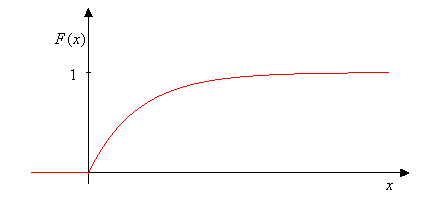
\includegraphics[scale=0.75]{pic/distrib.png}
                \caption{Příklad průběhu distribuční funkce exponenciálního rozdělení} \label{Obrázek č. 2.1}
            \end{figure}
        \subsubsection{Vlastnosti distribuční funkce}
            \begin{itemize} 
                \item
                Hodnoty distribuční funkce leží v intervalu od nuly do jedné.
                $$ 0 \leq F(x) \leq 1 $$
                \item
                Distribuční funkce je neklesající.
                $$  P(x_{1} \leq X < x_{2}) = F(x_{2}) - F(x_{1})   pro x_{1} < x_{2} $$
                \item
                V záporném nekonečnu se blíží k nule, v kladném nekonečnu se blíží k jedné.
                $$ F(- ∞) = 0, F(∞) = 1 $$ 
            \end{itemize}

    \section{Exponenciální rozdělění}
        Toto rozdělení má spojitá náhodná veličina X, která představuje dobu čekání do nastoupení (poissonovského) náhodného jevu, 
        nebo délku intervalu (časového nebo délkového) mezi takovými dvěma jevy (např. doba čekání na obsluhu, vzdálenost mezi dvěma poškozenými místy na silnici, doba do poruchy).
        Závisí na parametru $ \lambda $, což je převrácená hodnota střední hodnoty doby čekání do nastoupení sledovaného jevu. \cite{7}

        Náhodná veličina X má exponenciální rozdělení Exp($ \lambda $) právě tehdy, když je hustota pravděpodobnosti dána vztahem:
        $$  f(x) = \left\{ \begin{array}{ll}
            0 & \mbox{pro }x<0 \\
            \lambda.e^{\lambda.x} & \mbox{pro }x\geq 1
            \end{array} \right. $$
            \begin{figure}[h]
                \centering
                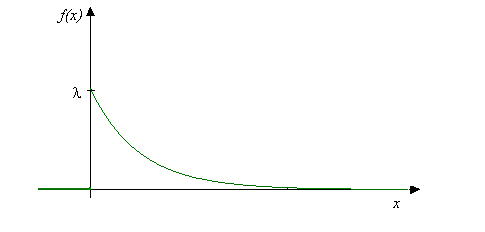
\includegraphics[scale=0.75]{pic/hustota.png}
                \caption{Příklad grafu hustoty pravděpodobnosti exponenciálního rozdělení} \label{Obrázek č. 2.1}
            \end{figure}

        \subsubsection*{Další vlastnosti}
        \begin{itemize} 
        \item
            $  F(x) = \left\{ \begin{array}{ll}
                0 & \mbox{pro }x<0 \\
                1-e^{-\lambda.x} & \mbox{pro }x\geq 1
                \end{array} \right. $
        \item
            $ E(x) = \frac{1}{\lambda}  $
        \item
            $ D(x) = \frac{1}{\lambda^{2}}  $

        \end{itemize}

    \section{Spolehlivost a střední doba mezi poruchami}
        \subsubsection{Střední doba mezi poruchami}
            Základní veličinou pro měření spolehlivosti systému je střední doba mezi poruchami (MTBF, Mean Time
            Between Failure). Obvykle je udávána v hodinách. Čím vyšší je hodnota MTBF, tím vyšší je spolehlivost
            produktu.\cite{3}
            Je statistická veličina používaná ke kvantifikaci spolehlivosti součásti, či celého výrobku.
            Určuje se pro výrobek nebo zařízení, které se opravuje. \cite{3}
        \subsubsection{Spolehlivost}
            Spolehlivost je schopnost systému nebo součásti vykonávat požadované funkce za daných
            podmínek po určené časové období \cite{4} 

            $$ Spolehlivost = e^{-(\frac{Doba}{MTBF})}$$

        \subsubsection{Pravděpodobnost bezporuchovosti}
            Značíme $ R(t) $. Udává pravděpodobnost, že výrobek do zadaného času $ t $ nebude mít poruchu. Jedná se o doplněk k hodnotě distribuční funkce $ F(t) $,
            což udává pravděpodobnost, že výrobek bude mít do času $ t $ poruchu.\cite{5}

            Pravděpodobnost bezporuchového provozu R(t) je dána vztahem:
            $$ R(t)=1-F(t) $$
   
    \section{Analýza blokového diagramu bezporuchovosti (RBD)}

        Analýza blokového diagramu bezporuchovosti (RBD - Reliability Block Diagram) je metoda analýzy systému. 
        Diagram RBD je grafická reprezentace logické struktury systému v podobě podsystémů, nebo jednotlivých součástí. 
        To umožňuje, aby byly cesty úspěchu (funkceschopného stavu) reprezentovány tak, jak jsou bloky (podsystémy/součásti) logicky propojeny.\cite{1}

        Blokové diagramy jsou mezi prvními úkoly dokončenými během etapy vymezení produktu. 
        Mají být vypracovány jako součást vývoje počáteční koncepce. 
        Práce na nich mají být zahájeny, jakmile existuje vymezení programu, a mají být dokončeny jako součást analýzy požadavků a 
        mají se neustále rozšiřovat do větších úrovní podrobnosti, 
        jakmile budou k dispozici data, aby bylo možné činit rozhodnutí a provádět optimalizace nákladů a přínosů.\cite{2}

    \section{Základní zapojení bloků}
        \subsubsection*{Sériové zapojení}
            Při poruše jedné komponenty dojde k poruše celého systému. 
            Systém je v bezporuchovém stavu, pokud všechny jeho komponenty nemají poruchu.\cite{5}
            Pravděpodobnost, že všechny komponenty (n) v sériovém systému budou mít poruchu je dána vztahem:
            $$ R = R_{1}R_{2}...R_{n} = e^{-\lambda_{1}t}e^{-\lambda_{2}t}...e^{-\lambda_{n}t} = e^{-(\lambda_{1} + \lambda_{2} + ... +\lambda_{n})t} $$
            \begin{figure}[h]
                \centering
                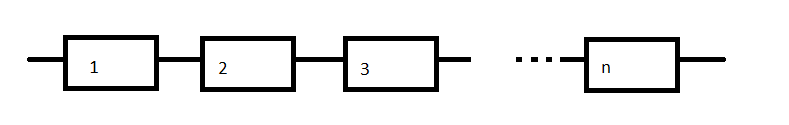
\includegraphics[scale=0.75]{pic/seriove.png}
                \caption{Příklad sériového zapojení komponent} \label{Obrázek č. 2.1}
            \end{figure}

        \subsubsection*{Paralelní zapojení}
            K poruše celého systemu dochází pokud jsou v poruše všechny jeho komponenty. Bezporuchový stav trvá, dokud je alespoň jedna komponenta v bezporuchovém stavu.
            Z hlediska odhadu pravděpodobnosti představuje paralelní systém nejlepší variantu pro odhad pravděpodobnosti bezporuchového stavu.
            Pravděpodobnost, že všechny komponenty (n) v paralelním systému budou mít poruchu je dána vztahem:
            $$ F = F_{1}F_{2}...F_{n} = (1-e^{-\lambda_{1}t})(1-e^{-\lambda_{2}t})...(1-e^{-\lambda_{n}t}) $$
            \begin{figure}[h]
                \centering
                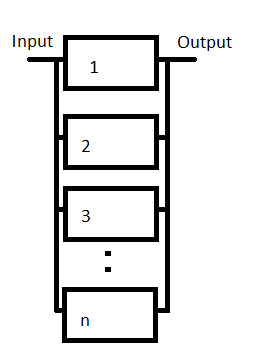
\includegraphics[scale=0.75]{pic/paralelni.png}
                \caption{Příklad paralelního zapojení kopmonent} \label{Obrázek č. 2.1}
            \end{figure}

\chapter{Návrh desktopové aplikce .NET}
    \section{Objektová struktura}
        \subsubsection{Item}
            Instance třídy Item jsou základní datové struktury vyžadující název bloku a rozdělení pravděpodobnosti.
        \subsubsection{Block}
            Jedná se o hlavní stvební stavební prvek RBD diagramu. 
            Může reprezentovat pouze jednu komponentu, či kolekci paralelních komponent typu Item. 
            %Dále může obsahovat kolekci paralelních bloků.
        \subsubsection{IDistribution}
            Rozhraní pro rozdělení pravděpodobnosti, které je jedním z atributů objektů typu Item, či může být spočítáno v objektu typu Block.
        \subsubsection{ExponencialDistribution}
            Instance této třídy reprezentuje konkrétní rozdělení pravděpodobnosti. Každá komponenta obsahuje vlastní objekt rozdělení.

    \begin{figure}[h]
        \centering
        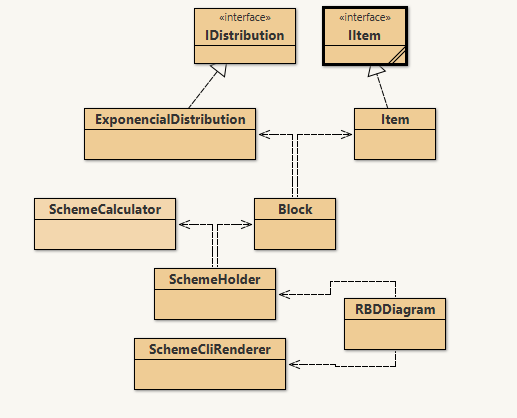
\includegraphics[scale=1]{pic/class.png}
        \caption{Zjednodušený class diagram nejčastěji používaných objektů} \label{Obrázek č. 2.1}
    \end{figure}
    
    \section{Pomocné třídy}
        SchemeHolder je objekt držící jednotlivé bloky v seznamu, tak jak byly vloženy. 
        SchemeCalculator je servisní třída, která má za úkol na základě předaných parametrů na uloženém schématu spočítat dílčí pravděpodobnosti bezporuchovosti jednotlivých komponent,
         tak i celkového diagramu.

\chapter{Průběh vývoje}
    \section{Rozdělení projektu na subprojekty}
        Celkové řešení je rozděleno na několik podprojektů, tak aby každý odpovídal svému účelu použití.
        \begin{itemize} 
        \item SpecianPRJ - projekt obsahující veškeré objektové struktury.
        \item SpecianPRJ.Cli - projekt zaměřený na manuální testování navržených struktur.
        \item SpecianPRJ.Gui - grafické uživatelské rozhraní pro výslednou aplikaci.
        \item SpecianPRJ.Tests - unit testy pro výpočty pravděpodobnosti na exponenciálním rozdělení.
        \end{itemize}
    \section{Zjednodušení diagramu}
        Pro zjednodušení tvorby diagramu bylo zavedeno pravidlo, že se systém skládá pouze ze série bloků, z nichž některé mohou reprezentovat paralelní zapojení.
        V aplikaci nelze vytvořit diagram obsahující vazby mezi bloky, které spolu bezprostředně nesousedí.
        \begin{figure}[h]
            \centering
            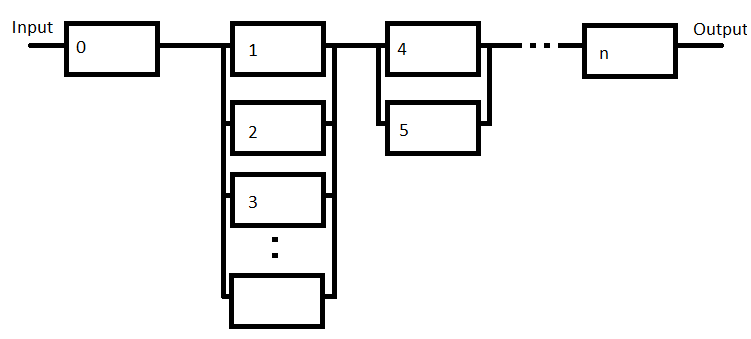
\includegraphics[scale=0.75]{pic/moznosti.png}
            \caption{Možnosti tvorby diagramu} \label{Obrázek č. 2.1}
    \end{figure}
    \section{Testování}
        Pro testování funkčních bloků byla použita výchozí knihovna pro Unit testování v prostředí .NET pro desktopové aplikace MSTest.
        Za pomoci testování jsem došel ke správným výsledkům za pomoci připravené konfigurace a tím jsem ušetřil práci manuálním testováním.
        Další nespornou výhodou testování je odhalení chyb při změně tím,  že testovací metody odhalí neočekávané výledky.

        Testované byly třídy pro výpočet distribuční funkce. Testování probíhá za pomoci zaokrouhlení na 6 desetinných míst.

\chapter{Návod k použití}

    Pro spuštění aplikace pro vývoj je potřeba mít nainstalované Visual Studio 2017 a novější. 
    V přiloženém CD ve složce SpecianPRJ spusťte soubor SpecianPRJ.sln. 

    Pro standartní spuštění aplikace stačí otevřít soubor SpecianPRJ.Gui.exe ve složce SpecianPRJ\\SpecianPRJ.Gui\\bin\\Debug.

    Pro obě varianty spuštní je nutným předpokladem nainstalovaný plný .NET Framework 4.6.1 a novější. 

    \section*{Založení nového diagramu}
    \section*{Uložení a otevření nového diagramu}
    \section*{Přidání prvku}
    \section*{Výpočty}

\chapter{Přehled existujících softwarových nástrojů}
    Zde uvedu seznam existujících softwarových řešení pro výpočty v oblasti pravděpodobnosti a teorie spolehlivosti, jejichž prospekty a ukázky jsem prošel.
    \begin{itemize} 
    \item ReliaSoft - analýza spolehlivosti
    \item Weibull.com - Reliability Analysis Software
    \item ItemSoft - Reliability Engineering Software
    \item AldService - Reliability Engineering
    \item Bqr - Leader in Reliability \& Maintenance Engineering and EDA
    \item Goldsim - Reliability Engineering and Risk Analysis for Complex Engineered Systems
    \item R Project - free software environment for statistical computing and graphics
    \end{itemize}

\chapter{Závěr}
    \section*{Dosažené výsledky}
    Ve vývojovém studiu Microsoft Visual Studio jsem vytvořil odpovídající projekt s rozdělenou strukturou podprojektů. 
    Seznámil jsem se s programovacím jazykem C\# a jeho základními objektovými principy. 
    Seznámil jsem se s teorií pravděpodobnosti a teorií spolehlivosti.
    Navrhl jsem jednoduchou objektovou strukturu, na níž jsem si vyzkoušel spočítat pravděpodobnost bezporuchovosti, 
    distribuční funkci pro exponenciální rozdělení a další potřebné charakteristiky.

    Na základě této objektové struktury jsem navrhl přehledné grafické rozhraní za pomoci knihoven WinForms, 
    ve kterém uživatel aplikace snadno nadefinuje strukturu komponent v sérii a může se na definovanou strukturu dotázat
    na pravděpodobnost bezporuchovosti v zadaném čase. Správnost výpočtů pravděpodobností a hodno distribuční funkce byla otestována za pomoci unit testů.

    Tvorba a zapojení komponent v RBD diagramu bylo zjednodušeno na sériový systém, kde jednotlivé komponenty mohou reprezentovat paralelní systém.

    Při vývoji aplikace jsem používal verzovací nástroj git, který mi umožnil si v různých větvích držet různé funkční a nefunkční cesty vývoje a spojovat do sebe různé
    věvte pro dosažení funkčního celku. \cite{8}

    \section*{Možnosti rozvoje aplikace}
    Aplikace nenabízí možnost tvorby složitějších schémat a propojení komponent tak, aby diagram odpovídal reálnému zadání. 
    Pro takové vylepšení by bylo nutné předělat objektový model včetně výpočetního postupu.
    Dále by bylo vhodné k aplikaci přidat možnost uložení a znovuotevírání uložených diagramů, 
    nyní je aplikace pouze demonstrační a diagram je nutné manuálně vytvořit po spuštění.

    Pro grafické uživatelské rozhraní by bylo vhodné přejít na knihovny WPF, které jsou nástupcem zastaralých Windows Forms.



\begin{thebibliography}{Mm99}
    \bibitem{1}
        28.6.2007, Prof. Ing. Václav Legát, DrSc., Zdroj: Verlag Dashöfer
    \bibitem{2}
        %https://theses.cz/id/dnvmwp/downloadPraceContent_adipIdno_11870
    \bibitem{3}
        http://gabben.wbs.cz/mtbf1.pdf
    \bibitem{4}
        IEEE 90
    \bibitem{5}
        %file:///C:/Users/King/Documents/PRJ/skripta/Plzen_06_10_2005.pdf
    \bibitem{6}
        https://homen.vsb.cz/~oti73/cdpast1/KAP03/PRAV3.HTM
    \bibitem{7}
        https://homen.vsb.cz/~oti73/cdpast1/KAP05/PRAV5.HTM
    \bibitem{8}
        We bring the awesome Git SCM to Windows. Git for windows [online]. [cit.2019-04-24]. Dostupné z: https://gitforwindows.org/
\end{thebibliography}

\end{document}
